\subsubsection{Convection in a 3d box}
\label{sec:cookbooks-simple-box-3d}

The world is not two-dimensional. While the previous section introduced a number
of the knobs one can play with with \aspect{}, things only really become
interesting once one goes to 3d. The setup from the previous section is easily
adjusted to this and in the following, let us walk through some of the changes
we have to consider when going from 2d to 3d. The full input file that
contains these modifications and that was used for the simulations we will show
subsequently can be found at \url{cookbooks/convection\_box\_3d.prm}.

The first set of changes has to do with the geometry: it is three-dimensional,
and we will have to address the fact that a box in 3d has 6 sides, not the 4 we
had previously. The documentation of the ``box'' geometry
(see Section~\ref{parameters:Geometry_20model}) states that these sides are
numbered as follows: ``\textit{in 3d, boundary indicators 0 through 5 indicate
left, right, front, back, bottom and top boundaries}.'' Recalling that we want
tangential flow all around and want to fix the temperature to known values at
the bottom and top, the following will make sense:
\lstinputlisting[language=prmfile]{start.part.prm.out}


The next step is to describe the initial conditions. As before, we will use an
unstably layered medium but the perturbation now needs to be both in $x$- and
$y$-direction
\lstinputlisting[language=prmfile]{initial.part.prm.out}

The third issue we need to address is that we can likely not afford a mesh as
fine as in 2d. We choose a mesh that is refined 3 times globally at the
beginning, then 3 times adaptively, and is then adapted every 15 time steps. We
also allow one additional mesh refinement in the first time step following
$t=0.003$ once the initial instability has given way to a more stable pattern:
\lstinputlisting[language=prmfile]{amr.part.prm.out}

Finally, as we have seen in the previous section, a computation with $Ra=10^4$
does not lead to a simulation that is exactly exciting. Let us choose $Ra=10^6$
instead (the mesh chosen above with up to 7 refinement levels after some time
is fine enough to resolve this). We can achieve this in the same way as in the
previous section by choosing $\alpha=10^{-10}$ and setting
\lstinputlisting[language=prmfile]{gravity.part.prm.out}
This has some interesting implications. First, a higher Rayleigh number makes
time scales correspondingly smaller; where we generated graphical output only
once every 0.01 time units before, we now need to choose the corresponding
increment smaller by a factor of 100:
\lstinputlisting[language=prmfile]{postprocess.part.prm.out}
Secondly, a simulation like this -- in 3d, with a significant number of cells,
and for a significant number of time steps -- will likely take a good amount of
time. The computations for which we show results below was run using 64
processors by running it using the command
{\tt{mpirun -n 64 ./aspect convection\_box\_3d.prm}}. If the machine should crash
during such a run, a significant amount of compute time would be lost if we had
to run everything from the start. However, we can avoid this by periodically
checkpointing the state of the computation:
\lstinputlisting[language=prmfile]{checkpoint.part.prm.out}
If the computation does crash (or if a computation runs out of the time limit
imposed by a scheduling system), then it can be restarted from such
checkpointing files (see the parameter {\tt Resume computation}
in Section~\ref{parameters:global}).
\index[prmindex]{Resume computation}
\index[prmindexfull]{Resume computation}

Running with this input file requires a bit of patience%
\footnote{For computations of this size, one should test a few time steps in
  debug mode but then, of course, switch to running the actual computation in
  optimized mode -- see Section~\ref{sec:debug-mode}.}
since the number of
degrees of freedom is just so large: it starts with a bit over 330,000\ldots
\begin{lstlisting}[frame=single,language=ksh]
Running with 64 MPI tasks.
Number of active cells: 512 (on 4 levels)
Number of degrees of freedom: 20,381 (14,739+729+4,913)

*** Timestep 0:  t=0 seconds
   Solving temperature system... 0 iterations.
   Rebuilding Stokes preconditioner...
   Solving Stokes system... 18 iterations.

Number of active cells: 1,576 (on 5 levels)
Number of degrees of freedom: 63,391 (45,909+2,179+15,303)

*** Timestep 0:  t=0 seconds
   Solving temperature system... 0 iterations.
   Rebuilding Stokes preconditioner...
   Solving Stokes system... 19 iterations.

Number of active cells: 3,249 (on 5 levels)
Number of degrees of freedom: 122,066 (88,500+4,066+29,500)

*** Timestep 0:  t=0 seconds
   Solving temperature system... 0 iterations.
   Rebuilding Stokes preconditioner...
   Solving Stokes system... 20 iterations.

Number of active cells: 8,968 (on 5 levels)
Number of degrees of freedom: 331,696 (240,624+10,864+80,208)

*** Timestep 0:  t=0 seconds
   Solving temperature system... 0 iterations.
   Rebuilding Stokes preconditioner...
   Solving Stokes system... 21 iterations.
[...]
\end{lstlisting}
\ldots{}but then increases quickly to around 2 million as the solution develops
some structure and, after time $t=0.003$ where we allow for an additional
refinement, increases to over 10 million where it then hovers between 8 and 14
million with a maximum of 15,147,534. Clearly, even on a reasonably quick
machine, this will take some time: running this on a machine bought in 2011,
doing the 10,000 time steps to get to $t=0.0219$ takes approximately 484,000
seconds (about five and a half days).

The structure or the solution is easiest to grasp by looking at isosurfaces of
the temperature. This is shown in Fig.~\ref{fig:box-3d-solution} and you can
find a movie of the motion that ensues from the heating at the bottom at
\url{http://www.youtube.com/watch?v=_bKqU_P4j48}. The simulation uses adaptively
changing meshes that are fine in rising plumes and sinking blobs and are coarse
where nothing much happens. This is most easily seen in the movie at
\url{http://www.youtube.com/watch?v=CzCKYyR-cmg}. Fig.~\ref{fig:box-3d-mesh}
shows some of these meshes, though still pictures do not do the evolving nature
of the mesh much justice. The effect of increasing the Rayleigh number is
apparent when comparing the size of features with, for example, the picture at
the right of Fig.~\ref{fig:convection-box-fields}. In contrast to that picture,
the simulation is also clearly non-stationary.

\begin{figure}
  \centering
  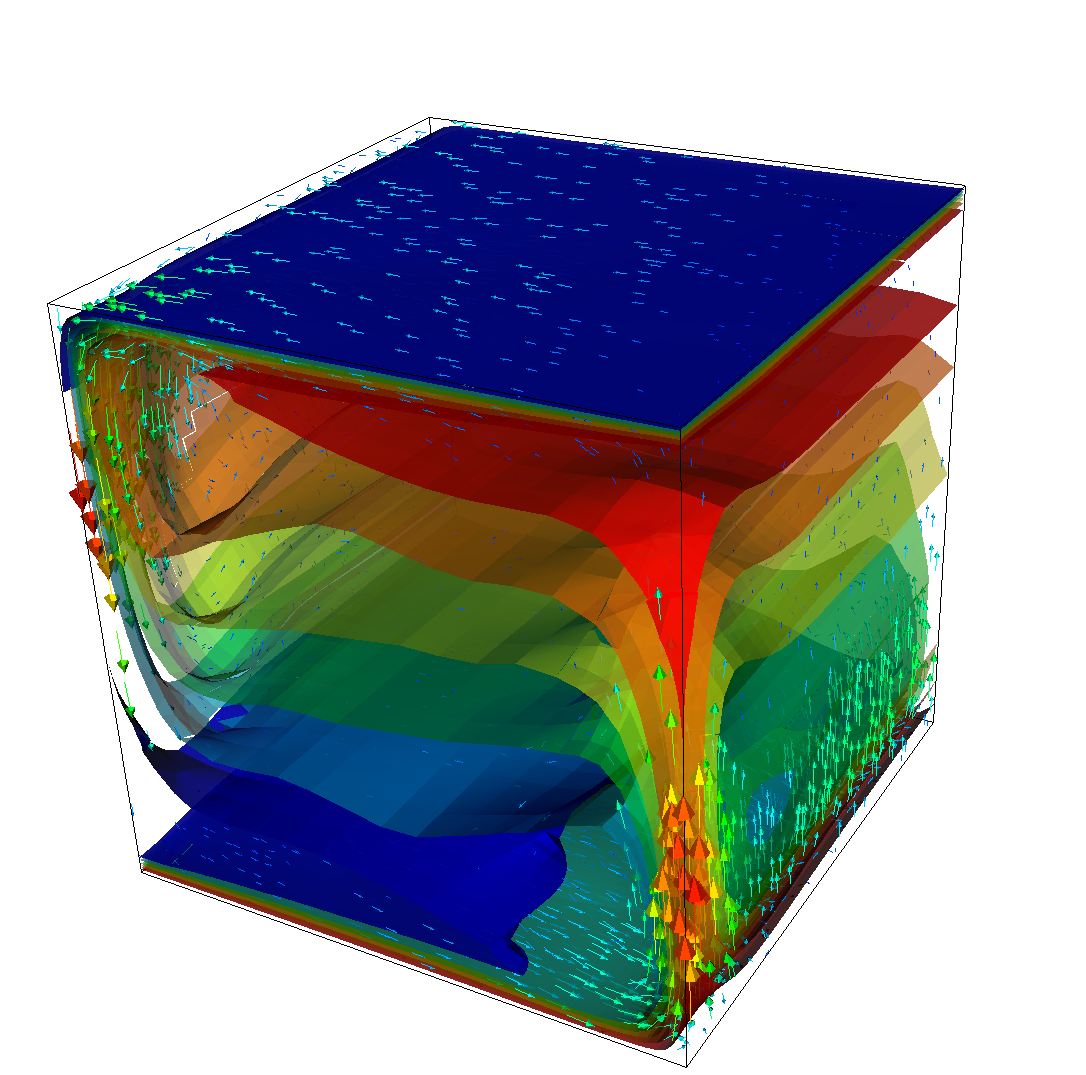
\includegraphics[width=0.3\textwidth]{movie0010.png}
  \hfill
  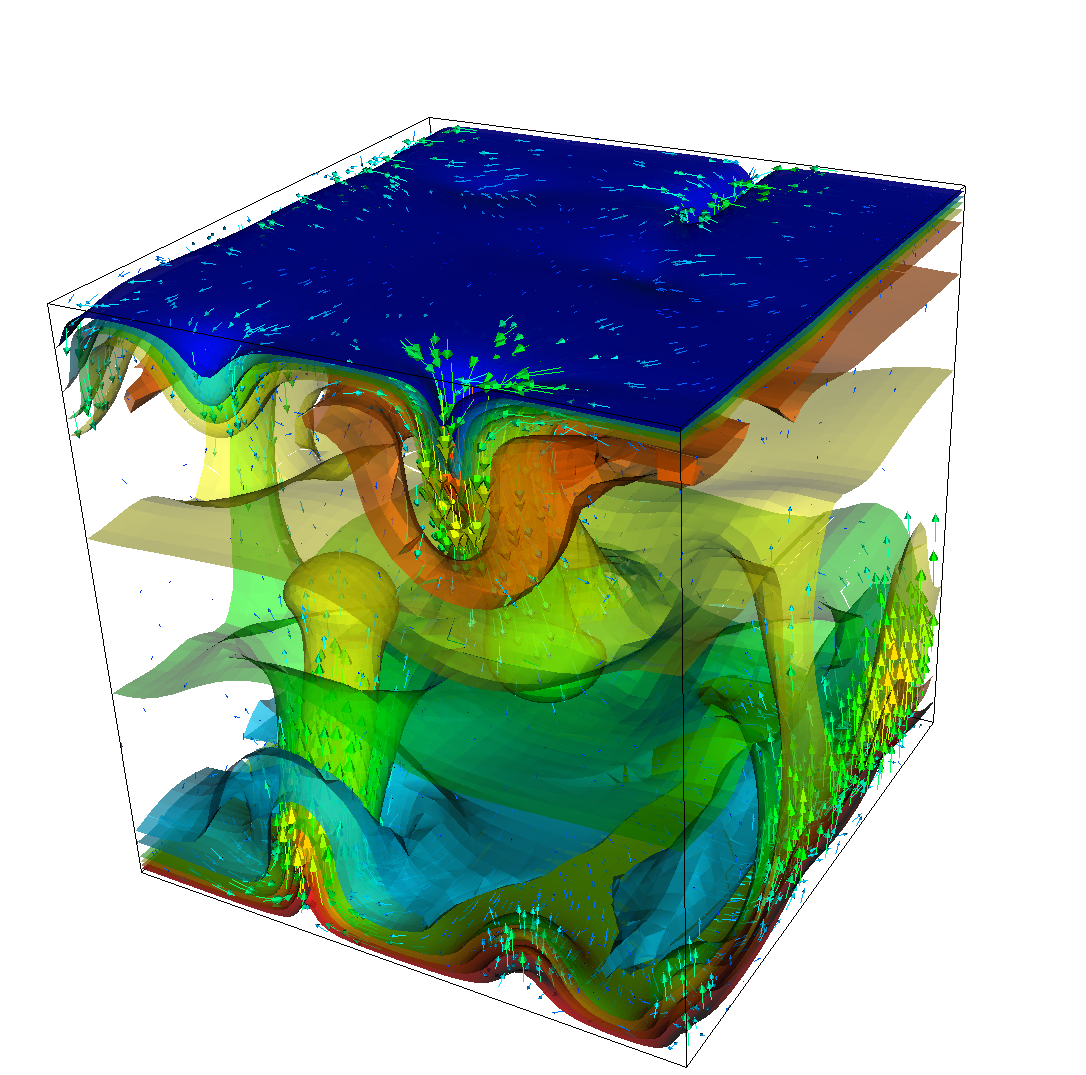
\includegraphics[width=0.3\textwidth]{movie0040.png}
  \hfill
  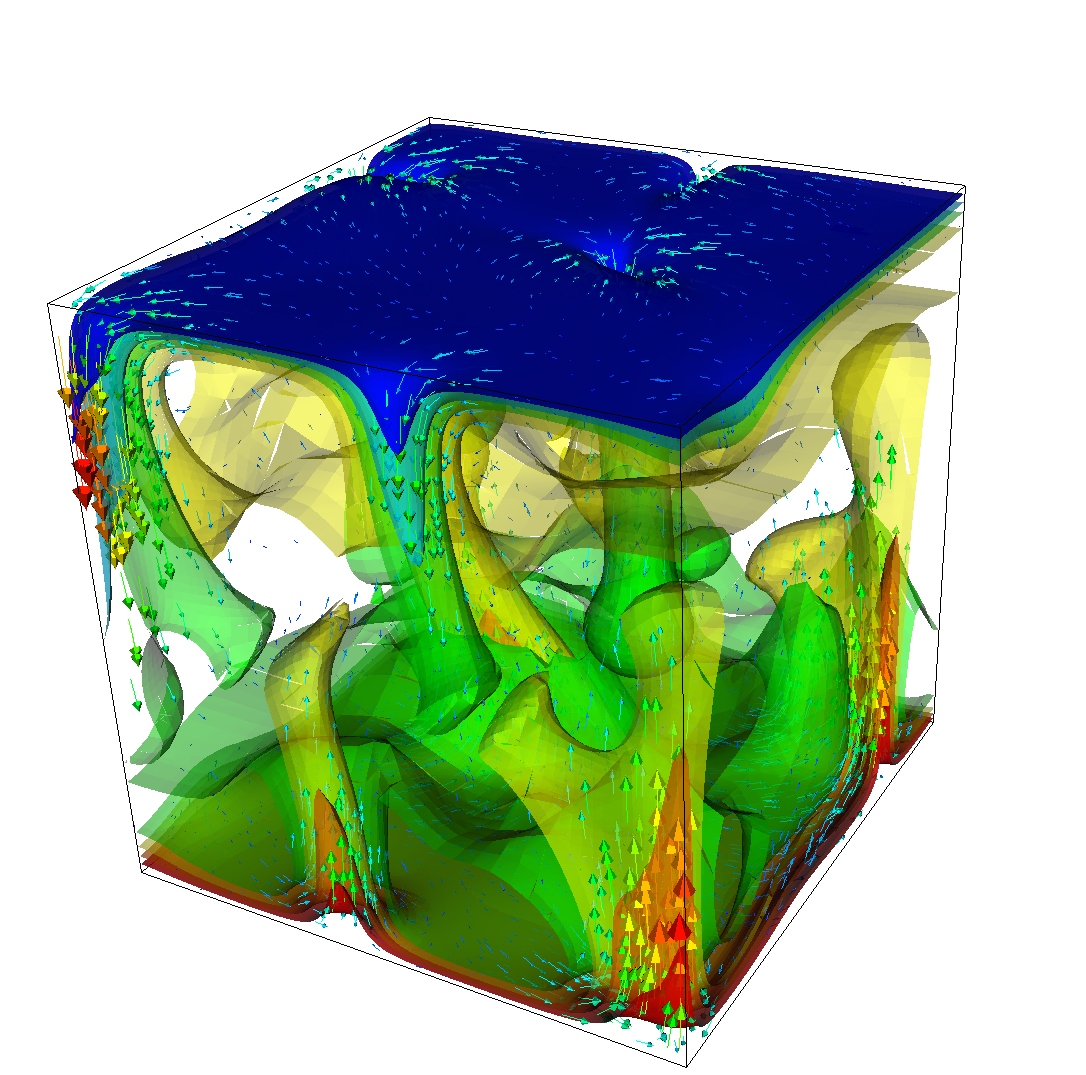
\includegraphics[width=0.3\textwidth]{movie0060.png}
  \\
  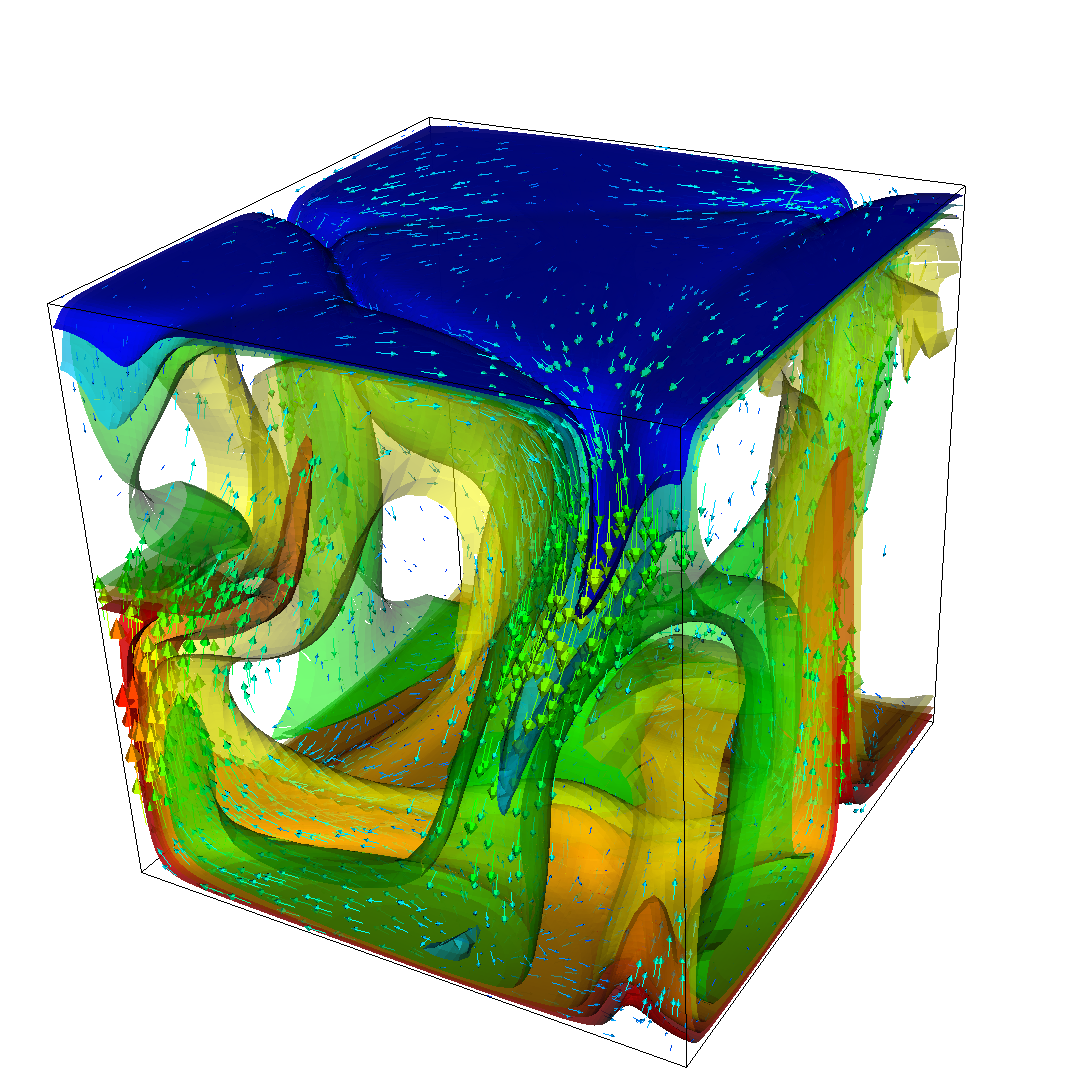
\includegraphics[width=0.3\textwidth]{movie0100.png}
  \hfill
  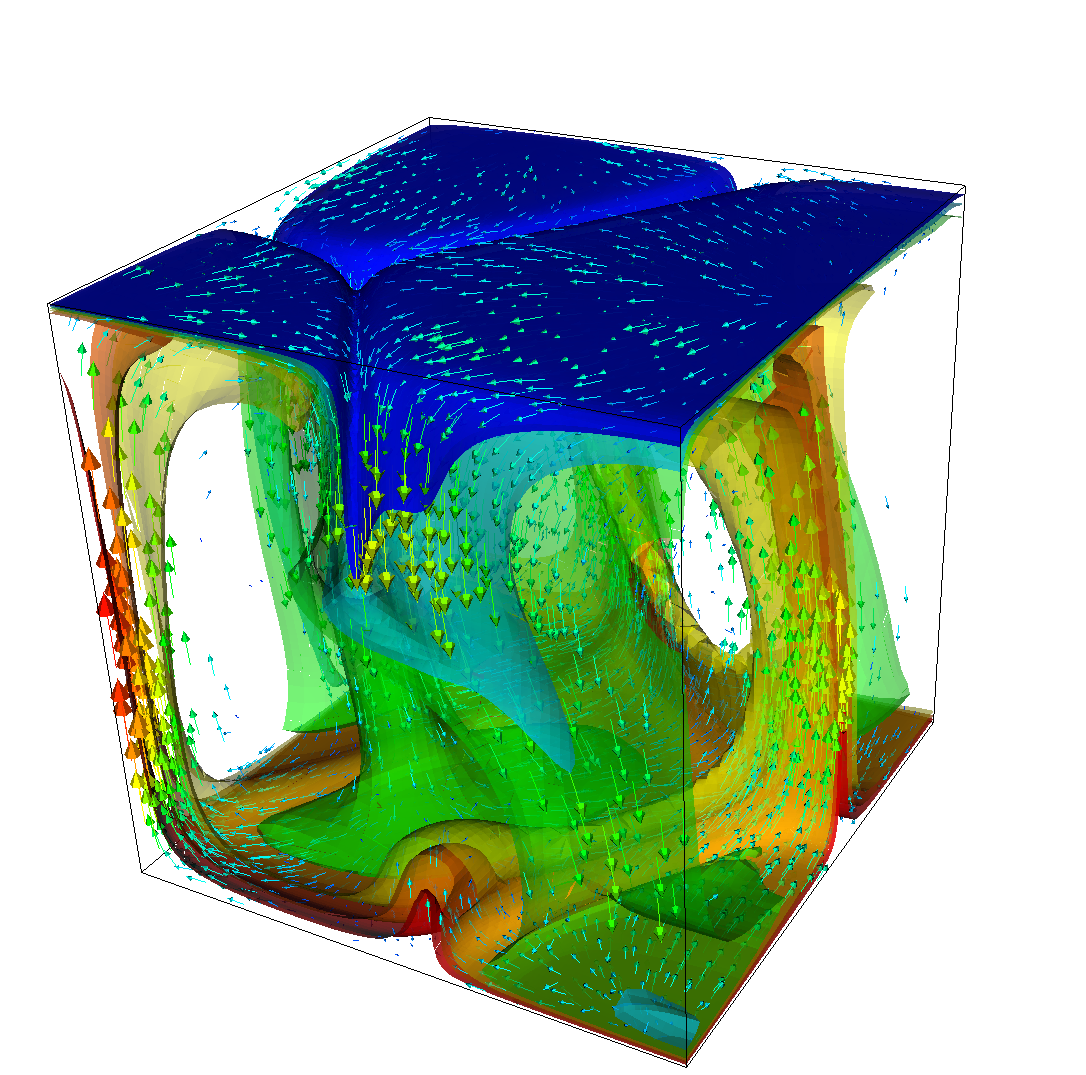
\includegraphics[width=0.3\textwidth]{movie0130.png}
  \hfill
  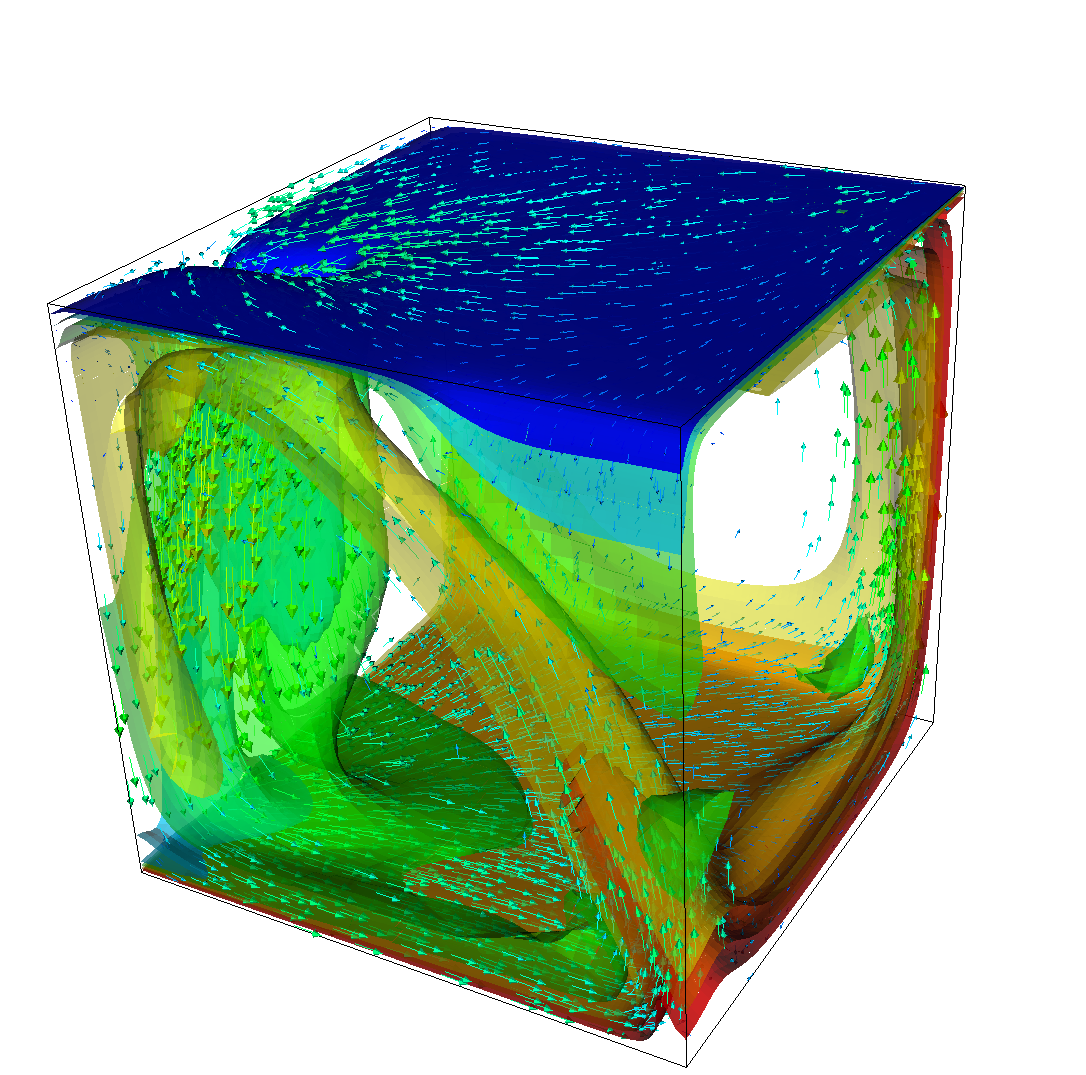
\includegraphics[width=0.3\textwidth]{movie0180.png}
  \caption{\it Convection in a 3d box: Temperature isocontours and some
  velocity vectors at the first time step after times $t=0.001, 0.004, 0.006$
  (top row, left to right) an $t=0.01, 0.013, 0.018$ (bottom row).}
  \label{fig:box-3d-solution}
\end{figure}


\begin{figure}
  \centering
  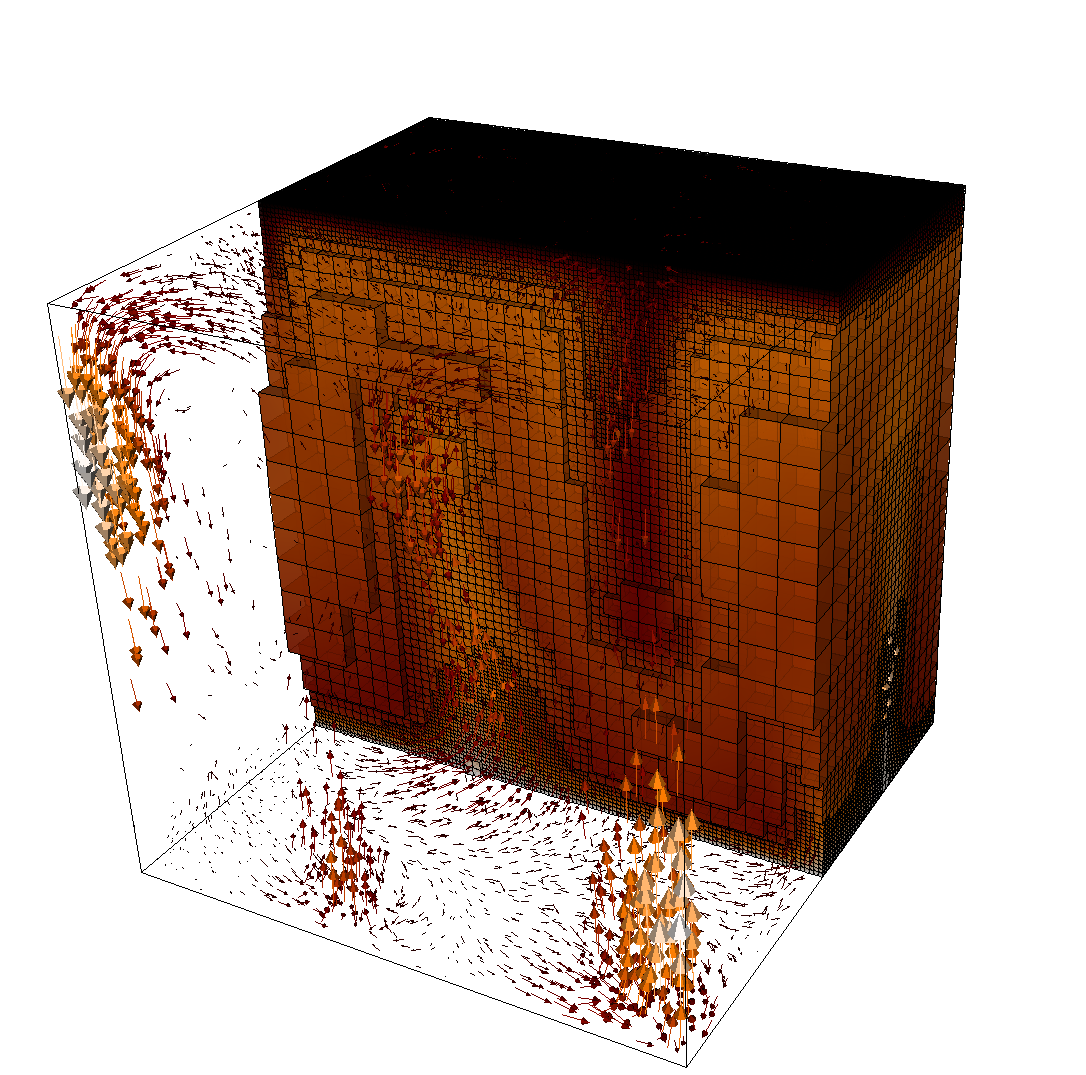
\includegraphics[width=0.3\textwidth]{mesh0060.png}
  \hfill
  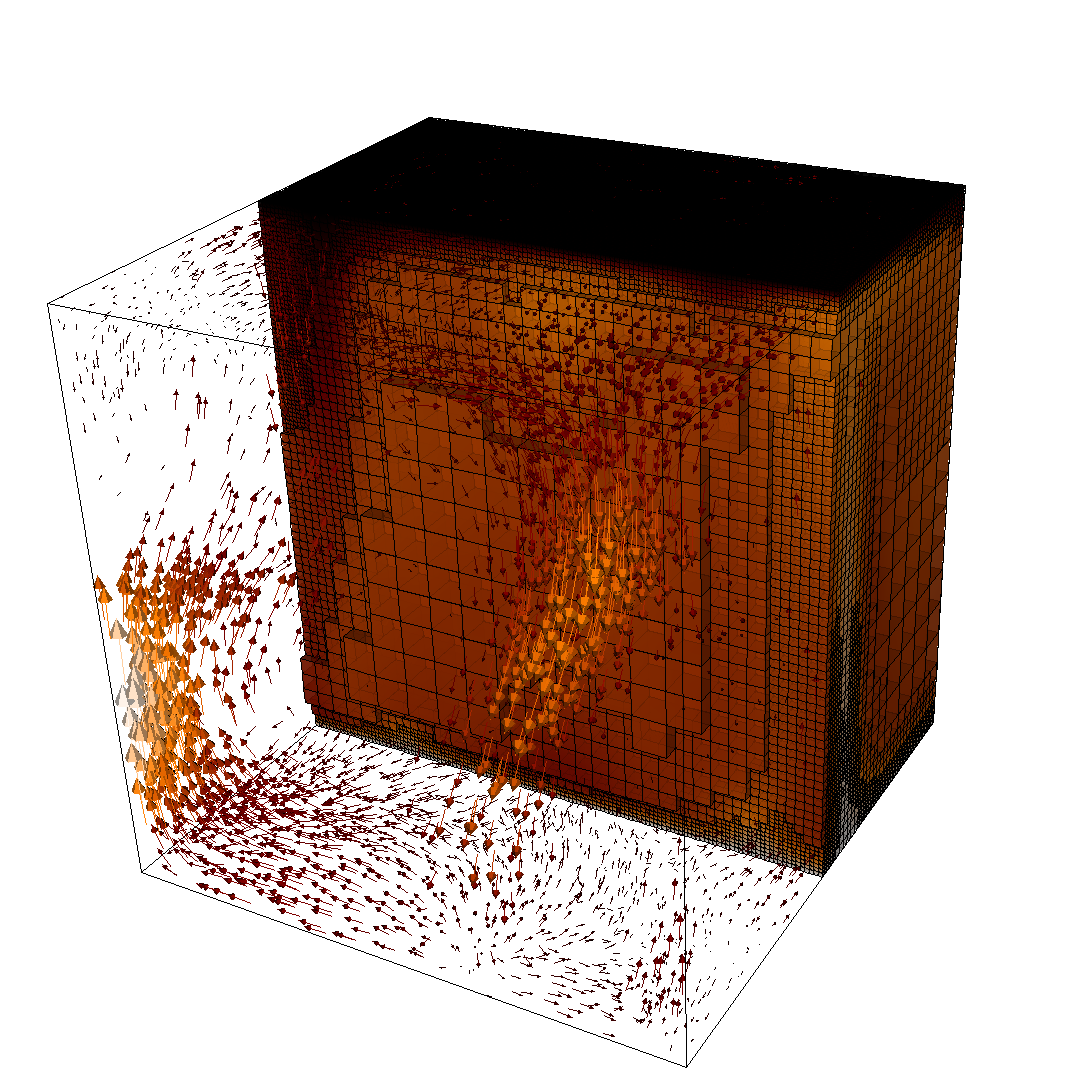
\includegraphics[width=0.3\textwidth]{mesh0100.png}
  \hfill
  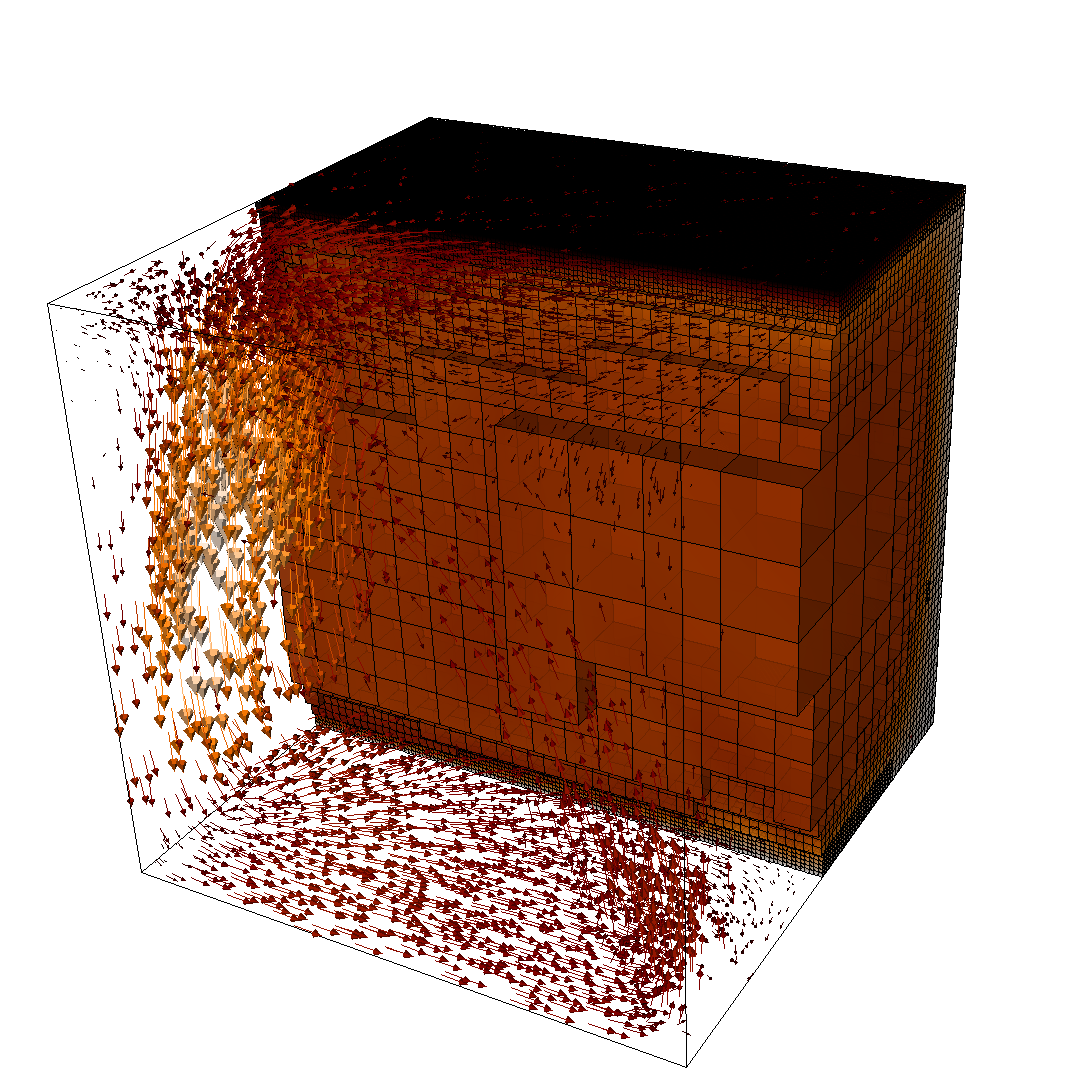
\includegraphics[width=0.3\textwidth]{mesh0180.png}
  \caption{\it Convection in a 3d box: Meshes and large-scale velocity field
  for the third, fourth and sixth of the snapshots shown in
  Fig.~\ref{fig:box-3d-solution}.}
  \label{fig:box-3d-mesh}
\end{figure}

As before, we could analyze all sorts of data from the statistics file but we
will leave this to those interested in specific data. Rather,
Fig.~\ref{fig:box-3d-heat-flux} only shows the upward heat flux through the
bottom and top boundaries of the domain as a function of time.%
\footnote{Note that the statistics file actually contains the \textit{outward}
heat flux for each of the six boundaries, which corresponds to the
\textit{negative} of upward flux for the bottom boundary. The figure therefore
shows the negative of the values available in the statistics file.}
The figure reinforces a pattern that can also be seen by watching the movie of
the temperature field referenced above, namely that the simulation can be
subdivided into three distinct phases. The first phase corresponds to the
initial overturning of the unstable layering of the temperature field and is
associated with a large spike in heat flux as well as large velocities (not
shown here). The second phase, until approximately $t=0.01$ corresponds to a
relative lull: some plumes rise up, but not very fast because the medium is now
stably layered but not fully mixed. This can be seen in the relatively low heat
fluxes, but also in the fact that there are almost horizontal temperature
isosurfaces in the second of the pictures in Fig.~\ref{fig:box-3d-solution}.
After that, the general structure of the temperature field is that the interior
of the domain is well mixed with a mostly constant average temperature and thin
thermal boundary layers at the top and bottom from which plumes rise and sink.
In this regime, the average heat flux is larger but also more variable depending
on the number of plumes currently active. Many other analyses would be possible
by using what is in the statistics file or by enabling additional
postprocessors.

\begin{figure}
  \centering
  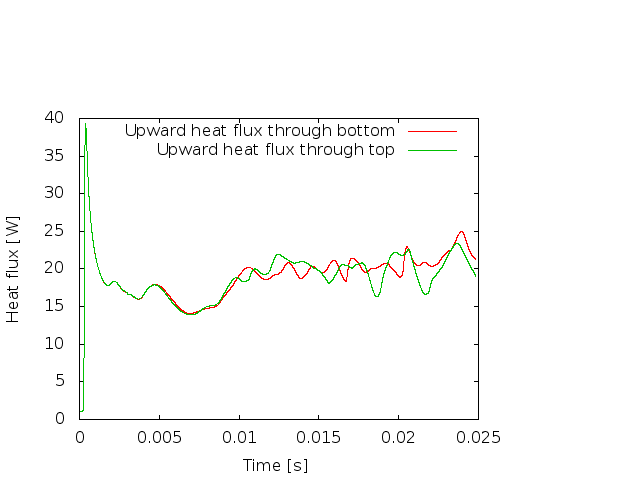
\includegraphics[width=0.6\textwidth]{heat-flux.png}
  \caption{\it Convection in a 3d box: Upward heat flux through the bottom and
  top boundaries as a function of time.}
  \label{fig:box-3d-heat-flux}
\end{figure}


